\label{chap.4}
%\section{Overview:}
The various deep learning algorithms that are explored are compared and evaluated through traditional classification metrics such as Accuracy, Precision, Recall and F1 score.
\section{Experimental Setup}

\subsection{Machine Learning and Deep Learning}
 The experiments are conducted using python. The machine learning library Scikit-Learn is used to train ML models such as SVM. The deep learning models are trained using the popular frameworks Tensorflow and PyTorch. 

 \

 The experiments are conducted on a system running of Ubuntu 22.04 (Pop OS with Nvidia proprietary Drivers). GPU acceleration is used to train the models faster. The models are trained over a time period of 2-6 hours on the whole dataset.


 \

 Hardware Specifications of the system Used include:
 i9 12th Generation Laptop processor
 Nvidia RTX 4070 GPU with 8GB VRAM 
 16 GB DDR5 RAM

\

The experiments used a custom dataset built using previously available public datasets and the data directly collected by our team. The dataset have a total of 17 classes with image samples of approximately 20,000. The class distribution of the dataset used is depicted in Figure 4.1.


\begin{figure}[h!]
    \centering
    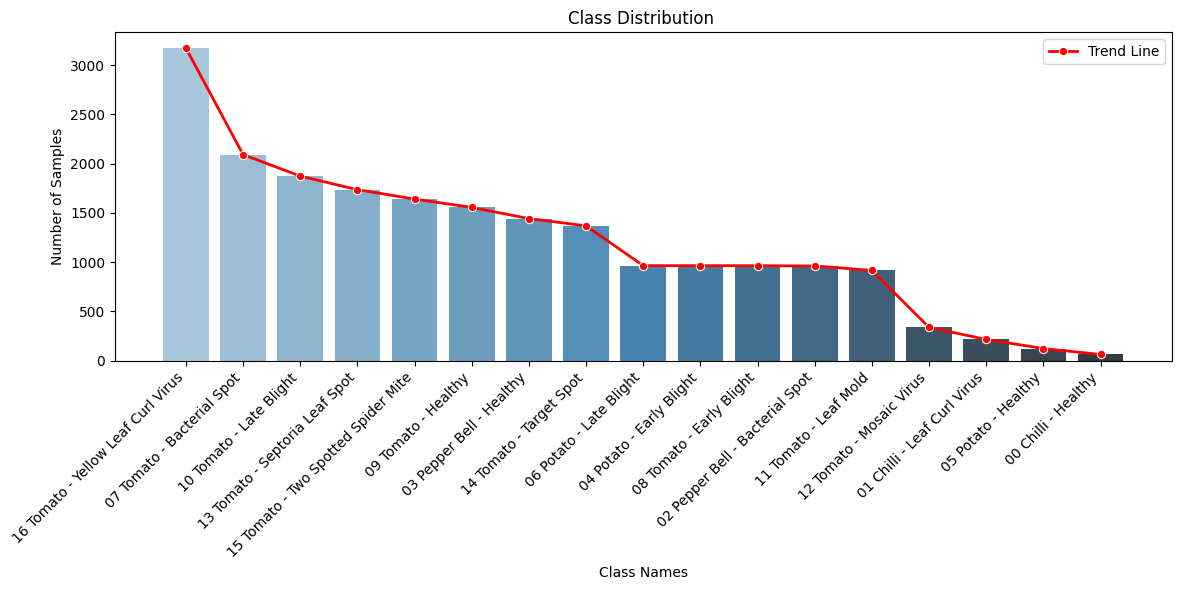
\includegraphics[scale=0.4]{ds_class_distribution.png}
    \caption{Class distribution of the dataset used for training}
    \label{fig:ds_class_distribution}
\end{figure}

\subsection{Development and Deployment}

The solutions that are explored are implemented as prototypes to test the accessibility and scalability. The developed prototypes are optimized for accessibility by ensuring development on cross platform compatible frameworks and languages. The performance and efficiency of the solutions are given top priority. The challenges due to constraints on the resources are overcome through intelligent architecture decisions.

\

Android application to access the solution under development is built using Flutter. This app is actively maintained to deliver the latest and most optimized experiences to the users. Most of the preprocessing of the captured or selected image is done in the app before uploading to decrease the deployment costs and enable a fast experience. The UI is designed to be intuitive and simple for everyone. An APK is built for each iteration of the application and is made available in the releases of the app's github repository. The application is then used to test the performance of the developed solution in the real world through our team at Coimbatore.

\

A website is built for improved accessibility and awareness. The website is built using React and deployed on the free tier static deployment of the Vercel platform.

\

The developed model is deployed on the cloud over the hugging face platform for free. The project follows a microservice architecture to decrease deployment costs and enable horizontal scaling based on demand.
There are two servers : 1) One for the vision model with the Vison Transformer. 
2) One to host the llama3.2 LLM for chat experience (experimental and not usable)
The servers are containerized using Docker.
The LLM server needs optimizations to better work on free hosting services that provide very limited computing power. The backend for the Vision model is written using Flask and the LLM's backend is written using llama.cpp utility for improved performance and low resource usage.





\section{Evaluation Metrics:}

\

the best developed model is then incorporated into the cloud for access through our mobile app. Then the app is tested and evaluated for basic usability based on criteria such as the prediction delay and latency. Then the app is used to test the model in real life conditions for user satisfaction through experts at Amrita Coimbatore Campus.

\

The development of the LLM is still in progress and its evaluation is done through real world usage in the supervision of experts to verify the responses.

\section{Experimental Design}
 
The baseline metrics that are to be improved on are decided using the analytical approach of feature extraction and training a basic Support Vector Machine using the extracted features. This is done only on the Chilli Leaf Curl Virus and the performance of the model is considered as baseline. The features extracted are the texture features.

\begin{figure}[h!]
    \centering
    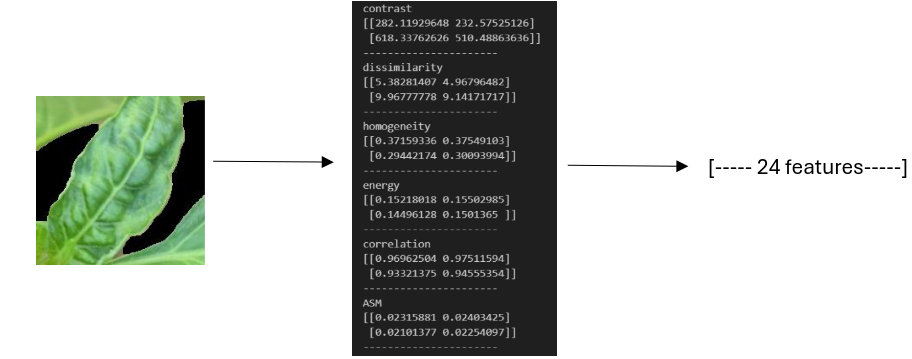
\includegraphics[scale=0.5]{svm_feature_extraction.png}
    \caption{feature extraction for SVM}
    \label{fig:svm_feature_extraction}
\end{figure}

\

\begin{table}[h!]
    \centering
    \begin{tabular}{|c|c|c|c|c|}
    \hline
    \textbf{Class} & \textbf{Precision} & \textbf{Recall} & \textbf{F1-Score} & \textbf{Support} \\ \hline
    0.0            & 0.86               & 0.86            & 0.86              & 7                \\ \hline
    1.0            & 0.86               & 0.86            & 0.86              & 7                \\ \hline
    \textbf{Accuracy}   & \multicolumn{3}{c|}{0.86}                         & 14               \\ \hline
    \textbf{Macro Avg}  & 0.86               & 0.86            & 0.86              & 14               \\ \hline
    \textbf{Weighted Avg} & 0.86               & 0.86            & 0.86              & 14               \\ \hline
    \end{tabular}
    \caption{Baseline SVM classification metrics}
    \label{tab:svm_classification_report}
\end{table}

\subsection{Experimental Scenarios:} 

Different Deep Learning Models are trained for solving the plant disease classification problem. Initially the popular DNN architectures of MobileNetV2, ResNet50, EfficientNetB0, InceptionV3 and DenseNet121 are trained for disease classification using the techniques of transfer learning. Then Attention based model of Vision Transformer is trained to be compared to the other models. The performances of these models are compared and contrasted for selection of a best model for deployment.

\subsection{Parameter Tuning:} 

Various techniques are used to improve the performance of the models and optimize hyperparameter for optimal performance. The preprocessing functions directly provided by the Tensorflow library are used to make sure the model works irrespective of the input size and shape. All the models are trained using a similar classification head over the base model. The classification head included Global Average Pooling 2D layer, a Dense layer with ReLU activation function followed by a Dropout Layer with a dropout rate of 0.5 and finally a dense layer with softmax activation for output.

\

The models used Adam Optimizer with sparse categorical crossentropy loss. Early stopping of training is used with validation loss as a monitor to avoid over-fitting. After each epoch the model is saved to prevent wastage of compute power. The best weights are restored according to performance on the validation step.

\

Learning rate scheduling is used to optimize the learning rate hyperparameter. The callback is built to automatically decrease the learning rate when the model is not improving or diverging.

\

All the models are compared over same test set for fair comparison of performance. 




\section{Results} 

All the metrics such as Precision, Recall and Accuracy are recorded for correct analysis and representation of the model performance. These results are calculated using the classfication-report function provided by the Scikit-Learn library. The confusion matrix is plotted for clear understanding of the model's performance, strengths and weaknesses.

\subsection{MobileNetV2}

The MobileNetV2 is trained in the mentioned conditions. The model recorded a trining speed of nearly 27ms per training step. When model is used for prediction of single images (without batch prediction), the model recorded a speed of approximately 50ms per image. 

\

The model got trained for a total of 34 epochs. The model was eventually stopped due to early stopping callback. The model's initial number of epochs is limited to 40. The model recorded a test accuracy of 91.84\%.

\begin{table}[h!]
    \centering
    \resizebox{\textwidth}{!}{%
    \begin{tabular}{|l|c|c|c|c|}
    \hline
    \textbf{Class}                                    & \textbf{Precision} & \textbf{Recall} & \textbf{F1-Score} & \textbf{Support} \\ \hline
    00 Chilli - Healthy                               & 1.00               & 0.52            & 0.69              & 23               \\ \hline
    01 Chilli - Leaf Curl Virus                       & 0.76               & 1.00            & 0.86              & 35               \\ \hline
    02 Pepper Bell - Bacterial Spot                   & 1.00               & 0.97            & 0.99              & 35               \\ \hline
    03 Pepper Bell - Healthy                          & 0.97               & 0.97            & 0.97              & 35               \\ \hline
    04 Potato - Early Blight                          & 0.97               & 0.97            & 0.97              & 35               \\ \hline
    05 Potato - Healthy                               & 1.00               & 0.89            & 0.94              & 28               \\ \hline
    06 Potato - Late Blight                           & 0.87               & 0.94            & 0.90              & 35               \\ \hline
    07 Tomato - Bacterial Spot                        & 0.94               & 0.94            & 0.94              & 35               \\ \hline
    08 Tomato - Early Blight                          & 0.81               & 0.74            & 0.78              & 35               \\ \hline
    09 Tomato - Healthy                               & 1.00               & 0.91            & 0.96              & 35               \\ \hline
    10 Tomato - Late Blight                           & 0.92               & 0.97            & 0.94              & 35               \\ \hline
    11 Tomato - Leaf Mold                             & 0.94               & 0.94            & 0.94              & 35               \\ \hline
    12 Tomato - Mosaic Virus                          & 1.00               & 0.97            & 0.99              & 35               \\ \hline
    13 Tomato - Septoria Leaf Spot                    & 0.94               & 0.91            & 0.93              & 35               \\ \hline
    14 Tomato - Target Spot                           & 0.86               & 0.89            & 0.87              & 35               \\ \hline
    15 Tomato - Two Spotted Spider Mite               & 0.82               & 0.91            & 0.86              & 35               \\ \hline
    16 Tomato - Yellow Leaf Curl Virus                & 0.95               & 1.00            & 0.97              & 35               \\ \hline
    \textbf{Accuracy}                                 & \multicolumn{3}{c|}{0.92}            & 576              \\ \hline
    \textbf{Macro Avg}                                & 0.93               & 0.91            & 0.91              & 576              \\ \hline
    \textbf{Weighted Avg}                             & 0.92               & 0.92            & 0.92              & 576              \\ \hline
    \end{tabular}%
    }
    \caption{Classification Report for MobileNetV2}
    \label{tab:classification_report_mnv2}
\end{table}

\subsection{ResNet50}

The ResNet50 model is trained in the mentioned conditions. The model recorded a trining speed of nearly 75ms per training step. When model is used for prediction of single images (without batch prediction), the model recorded a speed of approximately 75ms per image. 

\

The model got trained for a total of 38 epochs. The model was eventually stopped due to early stopping callback. The model's initial number of epochs is limited to 40. The model recorded a test accuracy of 94.27\% (Refer to Table 4.3).

\begin{table}[h!]
    \centering
    \resizebox{\textwidth}{!}{%
    \begin{tabular}{|l|c|c|c|c|}
    \hline
    \textbf{Class}                                    & \textbf{Precision} & \textbf{Recall} & \textbf{F1-Score} & \textbf{Support} \\ \hline
    00 Chilli - Healthy                               & 1.00               & 0.52            & 0.69              & 23               \\ \hline
    01 Chilli - Leaf Curl Virus                       & 0.76               & 1.00            & 0.86              & 35               \\ \hline
    02 Pepper Bell - Bacterial Spot                   & 1.00               & 0.97            & 0.99              & 35               \\ \hline
    03 Pepper Bell - Healthy                          & 0.97               & 1.00            & 0.99              & 35               \\ \hline
    04 Potato - Early Blight                          & 0.97               & 1.00            & 0.99              & 35               \\ \hline
    05 Potato - Healthy                               & 1.00               & 0.96            & 0.98              & 28               \\ \hline
    06 Potato - Late Blight                           & 0.97               & 1.00            & 0.99              & 35               \\ \hline
    07 Tomato - Bacterial Spot                        & 0.92               & 1.00            & 0.96              & 35               \\ \hline
    08 Tomato - Early Blight                          & 1.00               & 0.77            & 0.87              & 35               \\ \hline
    09 Tomato - Healthy                               & 0.95               & 1.00            & 0.97              & 35               \\ \hline
    10 Tomato - Late Blight                           & 0.92               & 0.97            & 0.94              & 35               \\ \hline
    11 Tomato - Leaf Mold                             & 0.94               & 0.94            & 0.94              & 35               \\ \hline
    12 Tomato - Mosaic Virus                          & 1.00               & 0.97            & 0.99              & 35               \\ \hline
    13 Tomato - Septoria Leaf Spot                    & 0.97               & 0.94            & 0.96              & 35               \\ \hline
    14 Tomato - Target Spot                           & 0.89               & 0.89            & 0.89              & 35               \\ \hline
    15 Tomato - Two Spotted Spider Mite               & 0.89               & 0.94            & 0.92              & 35               \\ \hline
    16 Tomato - Yellow Leaf Curl Virus                & 1.00               & 1.00            & 1.00              & 35               \\ \hline
    \textbf{Accuracy}                                 & \multicolumn{3}{c|}{0.94}            & 576              \\ \hline
    \textbf{Macro Avg}                                & 0.95               & 0.93            & 0.94              & 576              \\ \hline
    \textbf{Weighted Avg}                             & 0.95               & 0.94            & 0.94              & 576              \\ \hline
    \end{tabular}%
    }
    \caption{Classification Report for ResNet50}
    \label{tab:classification_report_rn50}
    \end{table}
    
\subsection{EfficientNetB0}

The EfficientNetB0 model is trained in the mentioned conditions. The model recorded a trining speed of nearly 35ms per training step. When model is used for prediction of single images (without batch prediction), the model recorded a speed of approximately 55ms per image. 

\

The model got trained for a total of 38 epochs. The model was eventually stopped due to early stopping callback. The model's initial number of epochs is limited to 40. The model recorded a test accuracy of 96.18\% (Refer to Table 4.4).

\begin{table}[h!]
    \centering
    \resizebox{\textwidth}{!}{%
    \begin{tabular}{|l|c|c|c|c|}
    \hline
    \textbf{Class}                                    & \textbf{Precision} & \textbf{Recall} & \textbf{F1-Score} & \textbf{Support} \\ \hline
    00 Chilli - Healthy                               & 1.00               & 0.70            & 0.82              & 23               \\ \hline
    01 Chilli - Leaf Curl Virus                       & 0.83               & 1.00            & 0.91              & 35               \\ \hline
    02 Pepper Bell - Bacterial Spot                   & 1.00               & 0.97            & 0.99              & 35               \\ \hline
    03 Pepper Bell - Healthy                          & 0.97               & 1.00            & 0.99              & 35               \\ \hline
    04 Potato - Early Blight                          & 0.97               & 0.94            & 0.96              & 35               \\ \hline
    05 Potato - Healthy                               & 1.00               & 0.96            & 0.98              & 28               \\ \hline
    06 Potato - Late Blight                           & 0.97               & 1.00            & 0.99              & 35               \\ \hline
    07 Tomato - Bacterial Spot                        & 1.00               & 1.00            & 1.00              & 35               \\ \hline
    08 Tomato - Early Blight                          & 0.97               & 0.91            & 0.94              & 35               \\ \hline
    09 Tomato - Healthy                               & 0.95               & 1.00            & 0.97              & 35               \\ \hline
    10 Tomato - Late Blight                           & 0.94               & 0.97            & 0.96              & 35               \\ \hline
    11 Tomato - Leaf Mold                             & 0.95               & 1.00            & 0.97              & 35               \\ \hline
    12 Tomato - Mosaic Virus                          & 1.00               & 0.94            & 0.97              & 35               \\ \hline
    13 Tomato - Septoria Leaf Spot                    & 0.97               & 0.97            & 0.97              & 35               \\ \hline
    14 Tomato - Target Spot                           & 0.97               & 0.89            & 0.93              & 35               \\ \hline
    15 Tomato - Two Spotted Spider Mite               & 0.92               & 1.00            & 0.96              & 35               \\ \hline
    16 Tomato - Yellow Leaf Curl Virus                & 1.00               & 1.00            & 1.00              & 35               \\ \hline
    \textbf{Accuracy}                                 & \multicolumn{3}{c|}{0.96}            & 576              \\ \hline
    \textbf{Macro Avg}                                & 0.97               & 0.96            & 0.96              & 576              \\ \hline
    \textbf{Weighted Avg}                             & 0.96               & 0.96            & 0.96              & 576              \\ \hline
    \end{tabular}%
    }
    \caption{Classification Report for EfficientNetB0}
    \label{tab:classification_report_en}
\end{table}


\subsection{InceptionV3}

The InceptionV3 model is trained in the mentioned conditions. The model recorded a trining speed of nearly 50ms per training step. When model is used for prediction of single images (without batch prediction), the model recorded a speed of approximately 64ms per image. 

\

The model got trained for full 40 epochs till limit. The model recorded a test accuracy of 85.24\% (Refer to Table 4.5).

\begin{table}[h!]
    \centering
    \resizebox{\textwidth}{!}{%
    \begin{tabular}{|l|c|c|c|c|}
    \hline
    \textbf{Class}                                    & \textbf{Precision} & \textbf{Recall} & \textbf{F1-Score} & \textbf{Support} \\ \hline
    00 Chilli - Healthy                               & 1.00               & 0.43            & 0.61              & 23               \\ \hline
    01 Chilli - Leaf Curl Virus                       & 0.74               & 1.00            & 0.85              & 35               \\ \hline
    02 Pepper Bell - Bacterial Spot                   & 0.92               & 0.94            & 0.93              & 35               \\ \hline
    03 Pepper Bell - Healthy                          & 0.97               & 0.94            & 0.96              & 35               \\ \hline
    04 Potato - Early Blight                          & 0.94               & 0.94            & 0.94              & 35               \\ \hline
    05 Potato - Healthy                               & 1.00               & 0.82            & 0.90              & 28               \\ \hline
    06 Potato - Late Blight                           & 0.83               & 0.97            & 0.89              & 35               \\ \hline
    07 Tomato - Bacterial Spot                        & 0.89               & 0.91            & 0.90              & 35               \\ \hline
    08 Tomato - Early Blight                          & 0.83               & 0.54            & 0.66              & 35               \\ \hline
    09 Tomato - Healthy                               & 0.94               & 0.94            & 0.94              & 35               \\ \hline
    10 Tomato - Late Blight                           & 0.79               & 0.94            & 0.86              & 35               \\ \hline
    11 Tomato - Leaf Mold                             & 0.79               & 0.77            & 0.78              & 35               \\ \hline
    12 Tomato - Mosaic Virus                          & 0.93               & 0.71            & 0.81              & 35               \\ \hline
    13 Tomato - Septoria Leaf Spot                    & 0.78               & 0.83            & 0.81              & 35               \\ \hline
    14 Tomato - Target Spot                           & 0.74               & 0.74            & 0.74              & 35               \\ \hline
    15 Tomato - Two Spotted Spider Mite               & 0.73               & 0.91            & 0.81              & 35               \\ \hline
    16 Tomato - Yellow Leaf Curl Virus                & 0.92               & 0.97            & 0.94              & 35               \\ \hline
    \textbf{Accuracy}                                 & \multicolumn{3}{c|}{0.85}            & 576              \\ \hline
    \textbf{Macro Avg}                                & 0.87               & 0.84            & 0.84              & 576              \\ \hline
    \textbf{Weighted Avg}                             & 0.86               & 0.85            & 0.85              & 576              \\ \hline
    \end{tabular}%
    }
    \caption{Classification Report for InceptionV3}
    \label{tab:classification_report_inv3}
\end{table}

\subsection{DenseNet121}

The DenseNet121 model is trained in the mentioned conditions. The model recorded a trining speed of nearly 68ms per training step. When model is used for prediction of single images (without batch prediction), the model recorded a speed of approximately 76ms per image. 

\

The model got trained for a total of 33 epochs. The model was eventually stopped due to early stopping callback. The model's initial number of epochs is limited to 40. The model recorded a test accuracy of 86.98\% (Refer to Table 4.6).

\begin{table}[h!]
    \centering
    \resizebox{\textwidth}{!}{%
    \begin{tabular}{|l|c|c|c|c|}
    \hline
    \textbf{Class}                                    & \textbf{Precision} & \textbf{Recall} & \textbf{F1-Score} & \textbf{Support} \\ \hline
    00 Chilli - Healthy                               & 0.00               & 0.00            & 0.00              & 23               \\ \hline
    01 Chilli - Leaf Curl Virus                       & 0.58               & 0.89            & 0.70              & 35               \\ \hline
    02 Pepper Bell - Bacterial Spot                   & 1.00               & 0.97            & 0.99              & 35               \\ \hline
    03 Pepper Bell - Healthy                          & 0.97               & 1.00            & 0.99              & 35               \\ \hline
    04 Potato - Early Blight                          & 0.94               & 0.94            & 0.94              & 35               \\ \hline
    05 Potato - Healthy                               & 1.00               & 0.50            & 0.67              & 28               \\ \hline
    06 Potato - Late Blight                           & 0.68               & 0.97            & 0.80              & 35               \\ \hline
    07 Tomato - Bacterial Spot                        & 0.92               & 0.97            & 0.94              & 35               \\ \hline
    08 Tomato - Early Blight                          & 0.89               & 0.71            & 0.79              & 35               \\ \hline
    09 Tomato - Healthy                               & 0.90               & 1.00            & 0.95              & 35               \\ \hline
    10 Tomato - Late Blight                           & 0.82               & 0.94            & 0.88              & 35               \\ \hline
    11 Tomato - Leaf Mold                             & 0.97               & 0.94            & 0.96              & 35               \\ \hline
    12 Tomato - Mosaic Virus                          & 1.00               & 0.94            & 0.97              & 35               \\ \hline
    13 Tomato - Septoria Leaf Spot                    & 0.87               & 0.94            & 0.90              & 35               \\ \hline
    14 Tomato - Target Spot                           & 0.80               & 0.80            & 0.80              & 35               \\ \hline
    15 Tomato - Two Spotted Spider Mite               & 0.91               & 0.91            & 0.91              & 35               \\ \hline
    16 Tomato - Yellow Leaf Curl Virus                & 0.97               & 0.97            & 0.97              & 35               \\ \hline
    \textbf{Accuracy}                                 & \multicolumn{3}{c|}{0.87}            & 576              \\ \hline
    \textbf{Macro Avg}                                & 0.84               & 0.85            & 0.83              & 576              \\ \hline
    \textbf{Weighted Avg}                             & 0.85               & 0.87            & 0.85              & 576              \\ \hline
    \end{tabular}%
    }
    \caption{Classification Report for DenseNet121}
    \label{tab:classification_report_dn121}
    \end{table}

\subsection{Google/ViT-base-patch16-224}

The ViT model is trained in the mentioned conditions. The model is more complex compared to the other models and the training and testing times are considerably higher. The model took about 3 hours to train and each image takes about 100ms to get a prediction.

The complexity and power pays off when it comes to performance and reliability. The model got a test accuracy of 99\% (Refer to table 4.7).

\begin{table}[h!]
    \centering
    \resizebox{\textwidth}{!}{%
    \begin{tabular}{|l|c|c|c|c|}
    \hline
    \textbf{Class}                                    & \textbf{Precision} & \textbf{Recall} & \textbf{F1-Score} & \textbf{Support} \\ \hline
    00 Chilli - Healthy                               & 0.95               & 0.87            & 0.91              & 23               \\ \hline
    01 Chilli - Leaf Curl Virus                       & 0.92               & 0.97            & 0.94              & 35               \\ \hline
    02 Pepper Bell - Bacterial Spot                   & 1.00               & 1.00            & 1.00              & 35               \\ \hline
    03 Pepper Bell - Healthy                          & 1.00               & 1.00            & 1.00              & 35               \\ \hline
    04 Potato - Early Blight                          & 0.97               & 1.00            & 0.99              & 35               \\ \hline
    05 Potato - Healthy                               & 0.97               & 1.00            & 0.98              & 28               \\ \hline
    06 Potato - Late Blight                           & 1.00               & 0.97            & 0.99              & 35               \\ \hline
    07 Tomato - Bacterial Spot                        & 1.00               & 1.00            & 1.00              & 35               \\ \hline
    08 Tomato - Early Blight                          & 1.00               & 0.97            & 0.99              & 35               \\ \hline
    09 Tomato - Healthy                               & 1.00               & 1.00            & 1.00              & 35               \\ \hline
    10 Tomato - Late Blight                           & 1.00               & 1.00            & 1.00              & 35               \\ \hline
    11 Tomato - Leaf Mold                             & 1.00               & 1.00            & 1.00              & 35               \\ \hline
    12 Tomato - Mosaic Virus                          & 1.00               & 1.00            & 1.00              & 35               \\ \hline
    13 Tomato - Septoria Leaf Spot                    & 1.00               & 1.00            & 1.00              & 35               \\ \hline
    14 Tomato - Target Spot                           & 1.00               & 1.00            & 1.00              & 35               \\ \hline
    15 Tomato - Two Spotted Spider Mite               & 1.00               & 1.00            & 1.00              & 35               \\ \hline
    16 Tomato - Yellow Leaf Curl Virus                & 1.00               & 1.00            & 1.00              & 35               \\ \hline
    \textbf{Accuracy}                                 & \multicolumn{3}{c|}{0.99}            & 576              \\ \hline
    \textbf{Macro Avg}                                & 0.99               & 0.99            & 0.99              & 576              \\ \hline
    \textbf{Weighted Avg}                             & 0.99               & 0.99            & 0.99              & 576              \\ \hline
    \end{tabular}%
    }
    \caption{Classification Report for Vision Transformer}
    \label{tab:classification_report}
\end{table}
    
\

The model got trained for a total of 33 epochs. The model was eventually stopped due to early stopping callback. The model's initial number of epochs is limited to 40. The model recorded a test accuracy of 86.98\% (Refer to Table 4.6).

\section{ Analysis of Results}
 Interpret the results and explain their significance.

\section{Observations:} Discuss patterns or anomalies observed in the results.
Example: "The proposed model outperforms baseline methods for dense graphs but shows reduced performance for sparse graphs."
Insights: Relate the results back to the research objectives and literature gaps.
Example: "The results validate the proposed hybrid approach's effectiveness in handling dynamic networks, addressing the scalability issue highlighted in the literature."
Statistical Significance (if applicable): Include significance testing to strengthen claims.
\section{ Comparative Analysis}
 Provide a side-by-side comparison of your results with those of existing methods.

Include a table summarizing metrics for all methods.
Discuss the relative advantages or limitations of your approach.
Example: "While the runtime of the proposed model is slightly higher than node2vec, it achieves significantly better precision."